\documentclass[tikz,border=0pt,11pt]{standalone}
\usepackage[T1]{fontenc}
\usepackage[utf8]{inputenc}
\usepackage{lmodern,amsmath,amssymb}
\usepackage[swedish]{babel}
\usetikzlibrary{arrows.meta,calc,positioning,decorations.pathmorphing,decorations.pathreplacing,patterns,shadings}
\definecolor{navy}{HTML}{102F40}
\definecolor{teal}{HTML}{147D78}
\definecolor{lightteal}{HTML}{E6F1ED}
\definecolor{gold}{HTML}{B88B3B}
\definecolor{palegold}{HTML}{F7EEDB}
\definecolor{rust}{HTML}{B6533B}
\definecolor{palerust}{HTML}{FAEAE4}
\definecolor{paper}{HTML}{F7F5EE}
\definecolor{muted}{HTML}{5B6D72}
\definecolor{line}{HTML}{D6DED8}
\renewcommand{\familydefault}{\sfdefault}
\newcommand{\atom}[5]{\shade[ball color=#3!70] (#1,#2) circle (#5);\node[text=white,font=\bfseries\small] at (#1,#2){#4};}
\newcommand{\water}[3]{\begin{scope}[shift={(#1,#2)},scale=#3]\draw[navy!45,line width=2pt] (-.3,.22)--(0,0)--(.3,.22);\atom{0}{0}{rust}{O}{.22}\atom{-.3}{.22}{teal}{H}{.15}\atom{.3}{.22}{teal}{H}{.15}\end{scope}}
\newcommand{\panel}[4]{\filldraw[fill=white,draw=line,rounded corners=5pt] (#1,#2) rectangle ++(#3,#4);}
\newcommand{\note}[4]{\node[txt,text width=#3cm] at (#1,#2){#4};}
\tikzset{txt/.style={anchor=north west,align=left,text=navy,font=\small},
 head/.style={anchor=west,text=navy,font=\bfseries\large},
 label/.style={align=center,text=navy,font=\small},
 smalllabel/.style={align=center,text=muted,font=\footnotesize},
 arrow/.style={-{Latex[length=2.5mm,width=1.8mm]},line width=1.2pt,draw=teal},
 goldarrow/.style={-{Latex[length=2.5mm]},line width=1.2pt,draw=gold},
 rustarrow/.style={-{Latex[length=2.5mm]},line width=1.2pt,draw=rust},
 dashedarrow/.style={arrow,dashed},
 badge/.style={fill=lightteal,rounded corners=3pt,text=teal,font=\bfseries\small,inner sep=5pt}}
\begin{document}
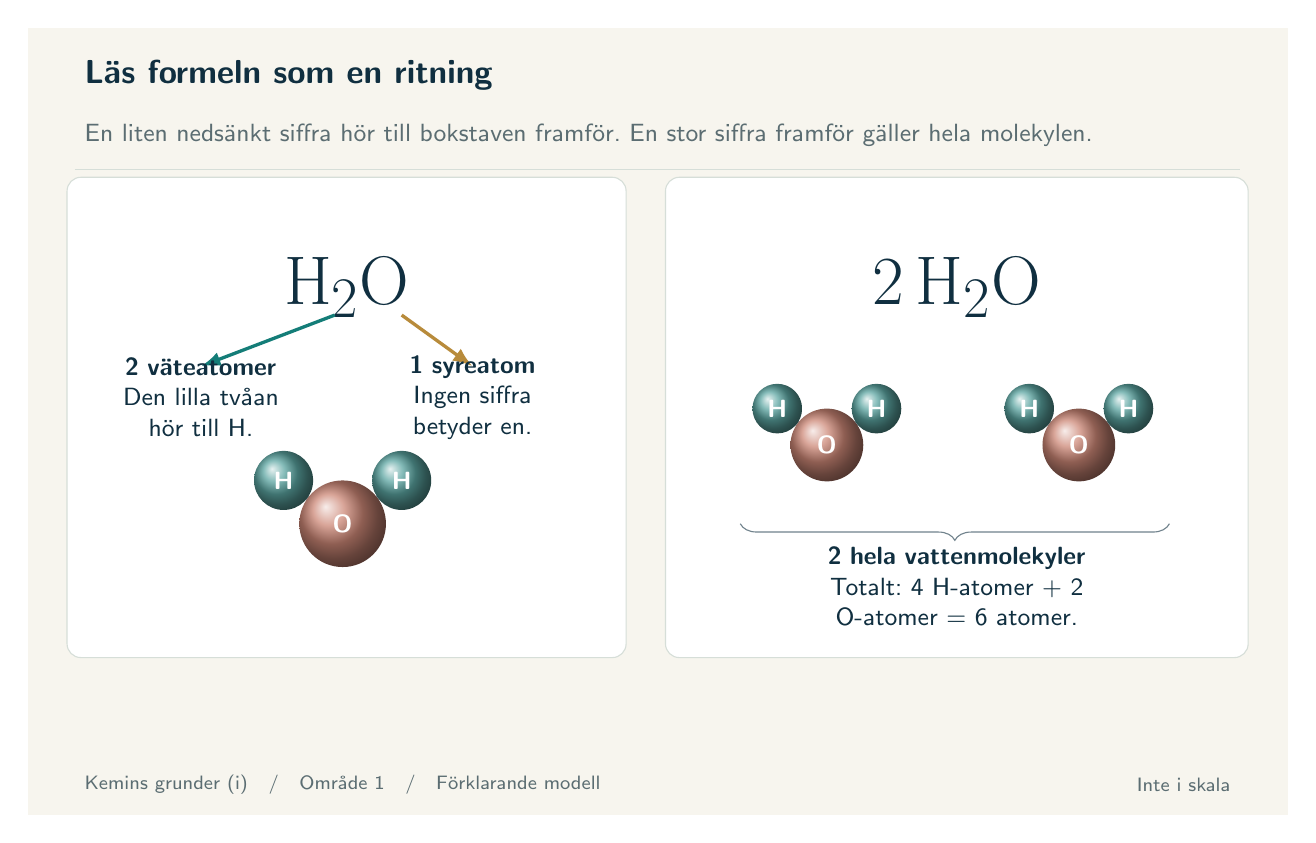
\begin{tikzpicture}[x=1cm,y=1cm]
\path[use as bounding box] (0,0) rectangle (16,10);
\fill[paper] (0,0) rectangle (16,10);
\node[head] at (.6,9.4){Läs formeln som en ritning};
\note{.6}{8.9}{14.8}{\textcolor{muted}{En liten nedsänkt siffra hör till bokstaven framför. En stor siffra framför gäller hela molekylen.}}
\draw[line] (.6,8.2)--(15.4,8.2);

\panel{.5}{2}{7.1}{6.1}\panel{8.1}{2}{7.4}{6.1}
\node[label,font=\bfseries\Huge] at (4.05,6.7){$\mathrm{H_2O}$};
\draw[arrow] (3.9,6.35)--(2.2,5.7);\draw[goldarrow] (4.75,6.35)--(5.65,5.7);
\node[label,text width=2.6cm] at (2.2,5.3){\textbf{2 väteatomer}\par Den lilla tvåan hör till H.};
\node[label,text width=2.8cm] at (5.65,5.3){\textbf{1 syreatom}\par Ingen siffra betyder en.};
\water{4}{3.7}{2.5}
\node[label,font=\bfseries\Huge] at (11.8,6.7){$2\,\mathrm{H_2O}$};
\water{10.15}{4.7}{2.1}\water{13.35}{4.7}{2.1}
\draw[decorate,decoration={brace,amplitude=6pt,mirror},navy!60] (9.05,3.7)--(14.5,3.7);
\node[label,text width=6cm] at (11.8,2.9){\textbf{2 hela vattenmolekyler}\par Totalt: 4 H-atomer + 2 O-atomer = 6 atomer.};\node[anchor=west,text=muted,font=\scriptsize] at (.6,.38){Kemins grunder (i)\quad /\quad Område 1\quad /\quad Förklarande modell};
\node[anchor=east,text=muted,font=\scriptsize] at (15.4,.38){Inte i skala};
\end{tikzpicture}\end{document}
